\chapter{The Duality Group \texorpdfstring{$O(d,d;\Z)$}{O(d,d;Z)}}\label{ch:odd}

On a circle, the closed string cannot tell the radius $R$ from $\ap/R$
(\cref{ch:tduality}). On a $d$-dimensional torus the background is a metric $G$ and a
two-form $B$, together $d^2$ real numbers (\cref{ch:narain}), and the corresponding question
is: \emph{which different pairs $(G,B)$ describe the same string physics?} The answer is a
group, the \emph{duality group}\index{duality group} $\Odd{d}$ of integer $2d\times2d$
matrices preserving the pairing between momentum and winding. This chapter defines the
group, shows why its defining condition is forced by level matching, describes three
families of elements with a direct physical meaning, and proves that two backgrounds related
by a group element have the same spectrum, state by state. That proof is short, it is
complete, and it has been checked in Lean; we give it on the page first and then compare
with the formal statement. The student should care for two reasons. First, the moduli space
of toroidal compactifications is the quotient of the space of pairs $(G,B)$ by this group,
so every statement about ``the space of string vacua on a torus'' depends on it. Second, the
whole of double field theory (\cref{ch:doubled,ch:genmetric,ch:dftaction}) is an attempt to
make the continuous version of this group manifest in a field theory.

%=====================================================================================
\section{What has to be explained}\label{sec:odd:setting}

\subsection{The data: charges, the generalized metric and the pairing}

We use the conventions of \cref{ch:narain}. The torus is $T^d=\R^d/2\pi\Z^d$ with
coordinates $X^i\sim X^i+2\pi$; the metric $G_{ij}$ (symmetric, positive definite) and the
Kalb--Ramond field $B_{ij}$ (antisymmetric) are constant and dimensionless, lengths being
measured in units of $\sqrt{\ap}$; and $E=G+B$ is the \emph{background
matrix}\index{background matrix}. A closed-string state carries $d$ integer winding numbers
$m^i$ and $d$ integer momentum numbers $n_i$. We collect them in the doubled charge vector
\begin{equation}\label{eq:odd:Z}
 Z=\begin{pmatrix}m\\ n\end{pmatrix}\in\Z^{2d},\qquad\text{windings first,}
\end{equation}
which is the ordering of Giveon, Porrati and Rabinovici \source{GPR §2.4, eq.~(2.4.18),
ll.~1278--1289} and of the Lean module \lean{DualScaleStream2/DFT/GeneralizedMetric.lean}.
Two matrices act on such vectors:
\begin{equation}\label{eq:odd:Heta}
 \HH(G,B)=\begin{pmatrix}G-BG^{-1}B&BG^{-1}\\[2pt]-G^{-1}B&G^{-1}\end{pmatrix},
 \qquad
 \eta=\begin{pmatrix}0&\mathbf 1_d\\ \mathbf 1_d&0\end{pmatrix},
\end{equation}
the generalized metric\index{generalized metric} \source{GPR §2.4, eq.~(2.4.17),
ll.~1266--1274} and the constant matrix that pairs momentum with winding. In terms of
them the mass formula and the level-matching condition\index{level matching} of
\cref{ch:narain} read
\begin{equation}\label{eq:odd:mass}
 \ap M^2=Z^{\mathsf T}\HH(G,B)\,Z+2\,(N+\tilde N-2),\qquad
 N-\tilde N=\tfrac12\,Z^{\mathsf T}\eta\,Z=n\cdot m ,
\end{equation}
where $N,\tilde N\in\{0,1,2,\dots\}$ are the oscillator levels of the two chiralities
\source{GPR §2.4, eqs.~(2.4.11), (2.4.16), (2.4.33), ll.~1183--1191, 1249--1256,
1459--1463}. The division of labour in \eqref{eq:odd:mass} is the key to the whole chapter:
\emph{the background enters only through $\HH$, and the constraint involves only $\eta$},
which knows nothing about the background.

It is useful to have the quadratic form written as a sum of squares. Because
$B^{\mathsf T}=-B$,
\begin{align}
 (n-Bm)^{\mathsf T}G^{-1}(n-Bm)
 &=n^{\mathsf T}G^{-1}n-2\,n^{\mathsf T}G^{-1}Bm+m^{\mathsf T}B^{\mathsf T}G^{-1}Bm\nonumber\\
 &=n^{\mathsf T}G^{-1}n-2\,n^{\mathsf T}G^{-1}Bm-m^{\mathsf T}BG^{-1}Bm ,\nonumber
\end{align}
and the two off-diagonal blocks of $\HH$ contribute
$m^{\mathsf T}BG^{-1}n-n^{\mathsf T}G^{-1}Bm=-2\,n^{\mathsf T}G^{-1}Bm$ (the first term is a
number, equal to its transpose $n^{\mathsf T}G^{-1}B^{\mathsf T}m$). Hence
\begin{equation}\label{eq:odd:squares}
 Z^{\mathsf T}\HH(G,B)\,Z=(n-Bm)^{\mathsf T}G^{-1}(n-Bm)+m^{\mathsf T}G\,m .
\end{equation}
The first term is the kinetic energy of the centre of mass, with the momentum shifted by the
$B$-field exactly as a vector potential shifts the momentum of a charged particle; the
second is the energy stored in the stretched string. Both are positive, so $\HH(G,B)$ is
positive definite.

\subsection{What a symmetry must do}

Suppose we relabel the charges by an integer matrix $g$, that is $Z\mapsto gZ$. For the
relabelling to lose no state and create none, $g$ must be a bijection of $\Z^{2d}$, so
$g^{-1}$ must also have integer entries. The relabelled state has mass form
\begin{equation}\label{eq:odd:covariance}
 (gZ)^{\mathsf T}\,\HH\,(gZ)=Z^{\mathsf T}\big(g^{\mathsf T}\HH\, g\big)Z .
\end{equation}
Read from right to left, this says: the numbers $Z^{\mathsf T}\HH'Z$ computed with the
matrix $\HH'=g^{\mathsf T}\HH g$ are the numbers $Z^{\mathsf T}\HH Z$ in a different order.
So the zero-mode energies of the backgrounds $\HH$ and $\HH'$ agree as lists, with
multiplicity, for \emph{every} invertible integer $g$. This is not yet a symmetry of the
string, because the physical states are those that satisfy the level-matching constraint in
\eqref{eq:odd:mass}, and the constraint must hold for $gZ$ if and only if it holds for $Z$
with the same $N-\tilde N$. We therefore need
\begin{equation}\label{eq:odd:polar}
 (gZ)^{\mathsf T}\eta\,(gZ)=Z^{\mathsf T}\eta\,Z\quad\text{for all }Z\in\Z^{2d}.
\end{equation}
The matrix $g^{\mathsf T}\eta g-\eta$ is symmetric, and a symmetric matrix $S$ with
$Z^{\mathsf T}SZ=0$ for all integer $Z$ vanishes: taking $Z$ a basis vector gives
$S_{II}=0$, and taking $Z$ the sum of two basis vectors gives $2S_{IJ}=0$. Condition
\eqref{eq:odd:polar} is therefore equivalent to the matrix equation
$g^{\mathsf T}\eta\,g=\eta$. This is the definition of the next section, and we have
found it by asking for nothing more than compatibility with level matching.

\begin{physicsbox}[Physical picture: two kinds of information]
The pairing $\eta$ is kinematics. It records that momentum and winding are conjugate
charges, and $\frac12Z^{\mathsf T}\eta Z=n\cdot m$ is the amount by which the left- and
right-moving oscillator levels must differ. It is the same for all tori. The generalized
metric $\HH$ is dynamics: it says how much energy a given charge costs on a given torus. A
duality is a relabelling of charges that respects the kinematics. It changes the dynamics
from $\HH$ to $g^{\mathsf T}\HH g$, and the theorem of this chapter is that the change is
invisible in the spectrum.
\end{physicsbox}

%=====================================================================================
\section{The groups \texorpdfstring{$\OddR{d}$}{O(d,d;R)} and
 \texorpdfstring{$\Odd{d}$}{O(d,d;Z)}}\label{sec:odd:group}

\begin{definition}\label{def:odd:group}
Let $\eta$ be the matrix in \eqref{eq:odd:Heta}. The group $\OddR{d}$\index{O(d,d;R)@$O(d,d;\R)$}
is the set of real $2d\times2d$ matrices $g$ with
\begin{equation}\label{eq:odd:def}
 g^{\mathsf T}\,\eta\,g=\eta ,
\end{equation}
and $\Odd{d}$\index{O(d,d;Z)@$O(d,d;\Z)$} is the subset of those with integer entries
\source{GPR §2.4, eqs.~(2.4.13)--(2.4.15), ll.~1213--1242, and ll.~1366--1367; AMN §3.1,
eq.~(3.4), ll.~569--601}.
\end{definition}

The name comes from the signature of $\eta$. For any $v\in\R^d$ the vectors $(v,v)$ and
$(v,-v)$ satisfy $\eta(v,\pm v)=\pm(v,\pm v)$, so $\eta$ has $d$ eigenvalues $+1$ and $d$
eigenvalues $-1$. In the basis of these eigenvectors $\eta$ becomes
$\diag(\mathbf 1_d,-\mathbf 1_d)$, and \eqref{eq:odd:def} is the definition of the
pseudo-orthogonal group of signature $(d,d)$, the analogue of the Lorentz group $O(1,3)$
with $d$ time-like and $d$ space-like directions. In the language of \cref{ch:narain} the
two eigenspaces are the left-moving and right-moving momenta at the point $G=\mathbf 1$,
$B=0$.

Writing $g$ in $d\times d$ blocks and multiplying out,
\begin{equation}\label{eq:odd:blocks}
 g=\begin{pmatrix}a&b\\c&d\end{pmatrix}:\qquad
 g^{\mathsf T}\eta g=\begin{pmatrix}a^{\mathsf T}c+c^{\mathsf T}a&a^{\mathsf T}d+c^{\mathsf T}b\\
 b^{\mathsf T}c+d^{\mathsf T}a&b^{\mathsf T}d+d^{\mathsf T}b\end{pmatrix},
\end{equation}
so that \eqref{eq:odd:def} is the set of three conditions
\begin{equation}\label{eq:odd:conditions}
 a^{\mathsf T}c+c^{\mathsf T}a=0,\qquad b^{\mathsf T}d+d^{\mathsf T}b=0,\qquad
 a^{\mathsf T}d+c^{\mathsf T}b=\mathbf 1
\end{equation}
\source{GPR §2.4, eq.~(2.4.15), ll.~1236--1242}; the fourth block is the transpose of the
third. (The letter $d$ denotes both the dimension and the lower-right block. This is the
notation of the literature, and the context always decides.)

\begin{proposition}[Group law and inverses]\label{prop:odd:group}
Let $g,h$ satisfy \eqref{eq:odd:def}. Then
\begin{enumerate}[label=(\roman*),itemsep=1pt]
\item $\eta^2=\mathbf 1$ and $\eta$ itself satisfies \eqref{eq:odd:def};
\item $gh$ satisfies \eqref{eq:odd:def};
\item $g$ is invertible, with $g^{-1}=\eta\,g^{\mathsf T}\eta$; if $g$ has integer entries,
 so has $g^{-1}$;
\item $g^{-1}$ and $g^{\mathsf T}$ satisfy \eqref{eq:odd:def}; equivalently
 $g\,\eta\,g^{\mathsf T}=\eta$;
\item $\det g=\pm1$.
\end{enumerate}
Consequently $\OddR{d}$ and $\Odd{d}$ are groups under matrix multiplication.
\end{proposition}
\begin{proof}
(i) $\eta^2=\mathbf 1$ is immediate from the block form, and then
$\eta^{\mathsf T}\eta\,\eta=\eta\,\eta\,\eta=\eta$ because $\eta$ is symmetric.
(ii) $(gh)^{\mathsf T}\eta(gh)=h^{\mathsf T}(g^{\mathsf T}\eta g)h=h^{\mathsf T}\eta h=\eta$.
(iii) Multiply \eqref{eq:odd:def} on the left by $\eta$:
$(\eta g^{\mathsf T}\eta)\,g=\eta^2=\mathbf 1$. A left inverse of a square matrix is a
two-sided inverse, so $g^{-1}=\eta g^{\mathsf T}\eta$, whose entries are those of $g$
rearranged:
\begin{equation}\label{eq:odd:inverse}
 g^{-1}=\eta\,g^{\mathsf T}\eta=\begin{pmatrix}d^{\mathsf T}&b^{\mathsf T}\\
 c^{\mathsf T}&a^{\mathsf T}\end{pmatrix}.
\end{equation}
(iv) From (iii), $g\,(\eta g^{\mathsf T}\eta)=\mathbf 1$; multiplying on the right by
$\eta$ gives $g\,\eta\,g^{\mathsf T}=\eta$, which is \eqref{eq:odd:def} for $g^{\mathsf T}$
\source{GPR §2.4, ll.~1244--1248}. For the inverse,
$(g^{-1})^{\mathsf T}\eta\,g^{-1}=(\eta g\eta)\,\eta\,(\eta g^{\mathsf T}\eta)
=\eta\,(g\,\eta\,g^{\mathsf T})\,\eta=\eta^3=\eta$.
(v) Take the determinant of \eqref{eq:odd:def}: $(\det g)^2\det\eta=\det\eta$ and
$\det\eta=(-1)^d\neq0$.
\end{proof}

No separate argument was needed for the integrality of $g^{-1}$. For a general integer
matrix the inverse involves a division by the determinant; here \eqref{eq:odd:inverse}
shows the inverse explicitly. This is the step that makes $Z\mapsto gZ$ a bijection of the
charge lattice and not only an injection.

\paragraph{How large is the group?} The real group is a Lie group. Writing
$g=\mathbf 1+\epsilon X$ in \eqref{eq:odd:def} and keeping first order in $\epsilon$ gives
$X^{\mathsf T}\eta+\eta X=0$, that is, $\eta X$ is antisymmetric. An antisymmetric
$2d\times2d$ matrix has $d(2d-1)$ independent entries, so
\begin{equation}\label{eq:odd:dim}
 \dim\OddR{d}=d(2d-1):\qquad 1,\;6,\;15,\;\dots\quad\text{for }d=1,2,3,\dots
\end{equation}
In blocks, $X=\left(\begin{smallmatrix}\alpha&\beta\\ \gamma&-\alpha^{\mathsf T}
\end{smallmatrix}\right)$ with $\alpha$ arbitrary ($d^2$ parameters) and $\beta,\gamma$
antisymmetric ($\frac12d(d-1)$ each). We shall meet the three kinds of block again as the
three kinds of finite transformation. The integer group $\Odd{d}$ is discrete; it is finite
for $d=1$ and infinite for $d\geq2$.

\begin{example}[The case $d=1$, completely]\label{ex:odd:d1}
For $d=1$ the blocks are numbers and \eqref{eq:odd:conditions} reads $2ac=0$, $2bd=0$,
$ad+bc=1$. If $c=0$ then $ad=1$ and hence $b=0$; if $a=0$ then $bc=1$ and hence $d=0$. So
\begin{equation}\label{eq:odd:O11R}
 O(1,1;\R)=\Big\{\begin{pmatrix}\lambda&0\\0&\lambda^{-1}\end{pmatrix},\
 \begin{pmatrix}0&\lambda\\ \lambda^{-1}&0\end{pmatrix}\ :\ \lambda\in\R\setminus\{0\}\Big\},
\end{equation}
a one-parameter group with four connected components, in agreement with \eqref{eq:odd:dim}.
With $\lambda=\ee^{\theta}$ the first family is the Lorentz boost of \cref{ch:narain} in
light-cone coordinates. Integer entries force $\lambda=\pm1$:
\begin{equation}\label{eq:odd:O11Z}
 O(1,1;\Z)=\{\mathbf 1,\,-\mathbf 1,\,\eta,\,-\eta\}\cong\Z_2\times\Z_2 .
\end{equation}
Here $\eta:(m,n)\mapsto(n,m)$ is the exchange of winding and momentum of
\cref{ch:tduality}, and $-\mathbf 1:(m,n)\mapsto(-m,-n)$ is the reflection $X\to-X$ of the
circle. \Cref{fig:odd:d1} shows the four-element orbit of a charge. The duality group of
the circle is small; the interesting structure starts at $d=2$.
\end{example}

\begin{figure}[t]
\centering
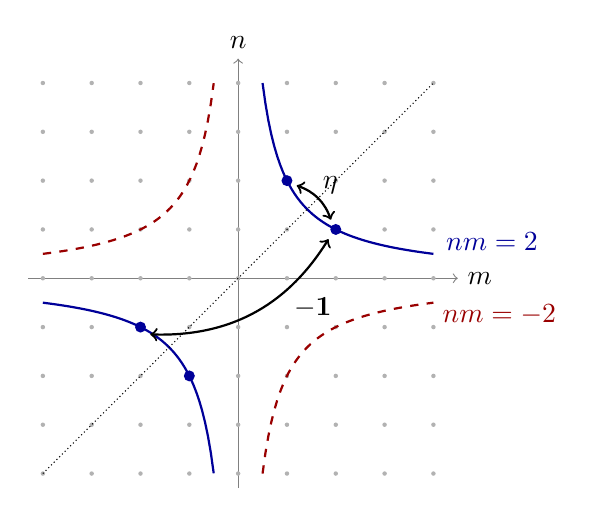
\begin{tikzpicture}[scale=0.62]
 \draw[->,gray] (-4.3,0)--(4.5,0) node[right,black] {$m$};
 \draw[->,gray] (0,-4.3)--(0,4.5) node[above,black] {$n$};
 \foreach \x in {-4,...,4} \foreach \y in {-4,...,4} \fill[gray!60] (\x,\y) circle (1.3pt);
 \draw[blue!60!black,thick,domain=0.5:4,samples=60] plot (\x,{2/\x});
 \draw[blue!60!black,thick,domain=-4:-0.5,samples=60] plot (\x,{2/\x});
 \draw[red!60!black,thick,dashed,domain=0.5:4,samples=60] plot (\x,{-2/\x});
 \draw[red!60!black,thick,dashed,domain=-4:-0.5,samples=60] plot (\x,{-2/\x});
 \draw[densely dotted] (-4,-4)--(4,4);
 \foreach \p in {(2,1),(1,2),(-2,-1),(-1,-2)} \fill[blue!60!black] \p circle (3.2pt);
 \draw[<->,thick] (1.9,1.2) to[bend right=25] node[above right=-2pt] {$\eta$} (1.2,1.9);
 \draw[<->,thick] (1.85,0.8) to[bend left=30] node[pos=0.3,below right=-1pt] {$-\mathbf 1$} (-1.8,-1.15);
 \node[blue!60!black] at (5.2,0.75) {$nm=2$};
 \node[red!60!black] at (5.35,-0.75) {$nm=-2$};
\end{tikzpicture}
\caption{The charge lattice of the circle, $d=1$. The level sets of
$\frac12Z^{\mathsf T}\eta Z=nm$ are hyperbolas; level matching places a state with
$N-\tilde N=2$ on the solid one. The group $O(1,1;\Z)$ has four elements and maps each
hyperbola to itself: $\eta$ is the reflection in the dotted diagonal and $-\mathbf 1$ the
reflection in the origin. The marked points are the orbit of $(m,n)=(2,1)$.}
\label{fig:odd:d1}
\end{figure}

\begin{pitfallbox}[Common pitfall: $O(d,d)$ is not $O(2d)$]
The condition is $g^{\mathsf T}\eta g=\eta$, not $g^{\mathsf T}g=\mathbf 1$. An element of
$\OddR{d}$ in general changes the Euclidean length $Z^{\mathsf T}Z$ of a charge vector, and
it changes $Z^{\mathsf T}\HH Z$ at fixed $\HH$; this is why a generic element of the
\emph{real} group maps a background to a physically different one \source{GPR §2.4,
ll.~1259--1262}. The elements of $\OddR{d}$ that are also orthogonal in the ordinary sense
form the compact subgroup $O(d)\times O(d)$ of rotations of left- and right-moving momenta
separately, which appeared in \cref{ch:narain} as the denominator of the moduli space.
\end{pitfallbox}

%=====================================================================================
\section{Dual backgrounds have the same spectrum}\label{sec:odd:spectrum}

We can now state and prove the main theorem. It is formulated for an arbitrary real
matrix $\HH$; that $g^{\mathsf T}\HH g$ is again the generalized metric of some
torus is a separate fact, proved in \cref{sec:odd:action}.

\begin{theorem}[Spectrum equivalence]\label{thm:odd:spectrum}
Let $g\in\Odd{d}$ and let $\HH$ be a real $2d\times2d$ matrix. Put
$\HH'=g^{\mathsf T}\HH\,g$. Then the map
\[
 e:\Z^{2d}\to\Z^{2d},\qquad e(Z)=gZ,
\]
is a bijection, and for every $Z\in\Z^{2d}$
\begin{equation}\label{eq:odd:spectrum}
 Z^{\mathsf T}\HH'Z=e(Z)^{\mathsf T}\,\HH\;e(Z),\qquad
 e(Z)^{\mathsf T}\,\eta\;e(Z)=Z^{\mathsf T}\eta\,Z .
\end{equation}
\end{theorem}
\begin{proof}
\emph{Bijection.} By \cref{prop:odd:group}(iii) the matrix $g^{-1}=\eta g^{\mathsf T}\eta$ has
integer entries, so $Z\mapsto g^{-1}Z$ maps $\Z^{2d}$ to itself and is a two-sided inverse
of $e$.
\emph{Mass form.} $e(Z)^{\mathsf T}\HH\,e(Z)=(gZ)^{\mathsf T}\HH(gZ)
=Z^{\mathsf T}g^{\mathsf T}\HH gZ=Z^{\mathsf T}\HH'Z$, which is \eqref{eq:odd:covariance}.
This step uses only the rule $(gZ)^{\mathsf T}=Z^{\mathsf T}g^{\mathsf T}$ and would hold
for any matrix $g$.
\emph{Charge norm.} $e(Z)^{\mathsf T}\eta\,e(Z)=Z^{\mathsf T}(g^{\mathsf T}\eta g)Z
=Z^{\mathsf T}\eta Z$ by \eqref{eq:odd:def}.
\end{proof}

The proof is three lines long because the work was done in choosing the variables. In
terms of $(G,B)$ the map $\HH\mapsto g^{\mathsf T}\HH g$ is a complicated non-linear
transformation, the Buscher rules of \cref{ch:buscher} being a special case, and a direct
check that the zero-mode Hamiltonian of \cref{ch:narain} is invariant would be laborious. In
terms of $\HH$ and $Z$ it is linear algebra.

\begin{corollary}[Full perturbative mass spectrum]\label{cor:odd:full}
Let $\HH=\HH(G,B)$ and suppose $\HH'=g^{\mathsf T}\HH g$ equals $\HH(G',B')$ for some
background $(G',B')$. Then the closed-string spectra \eqref{eq:odd:mass} on the two
backgrounds coincide, including multiplicities.
\end{corollary}
\begin{proof}
A state of the primed theory is labelled by a charge $Z$ and an oscillator state at levels
$(N,\tilde N)$ with $N-\tilde N=\frac12Z^{\mathsf T}\eta Z$. Assign to it the charge $e(Z)$
and the same oscillator occupation numbers in the unprimed theory. By
\eqref{eq:odd:spectrum} the constraint is again satisfied and $\ap M^2$ is the same. The
assignment is a bijection because $e$ is, and because the number of oscillator states at
given levels $(N,\tilde N)$ is a count of partitions that does not depend on the background
(\cref{ch:narain}; the oscillators obey
$[\alpha^i_k,\alpha^j_l]=k\,G^{ij}\delta_{k+l,0}$ for every $G$ \source{GPR §2.4,
eq.~(2.4.32), ll.~1446--1456}, and a change of $G$ is a change of basis in the space
they span).
\end{proof}

\begin{pitfallbox}[Common pitfall: equal spectra are necessary, not sufficient]
\Cref{thm:odd:spectrum} and its corollary compare lists of masses. Two quantum theories
with the same spectrum need not be the same theory; one must also match all correlation
functions. Giveon, Porrati and Rabinovici are explicit that the spectrum condition is only
``a necessary condition'', and that the equivalence of the theories is established
separately, by exhibiting the dualities as residual gauge symmetries \source{GPR §2.4,
ll.~1336--1348}. For the factorized dualities the path-integral derivation of
\cref{ch:buscher} provides such an argument on every worldsheet. In this chapter, and in the
Lean development, ``same spectrum'' means exactly the statement
\eqref{eq:odd:spectrum}.
\end{pitfallbox}

%=====================================================================================
\section{How the group acts on backgrounds}\label{sec:odd:action}

\Cref{thm:odd:spectrum} compares $\HH$ with $g^{\mathsf T}\HH g$. To read it as a statement
about tori we must know that $g^{\mathsf T}\HH(G,B)\,g$ is again of the form
$\HH(G',B')$, and we want a formula for $(G',B')$. Both follow from a characterization of
generalized metrics that does not mention $G$ and $B$.

\begin{lemma}[Which matrices are generalized metrics]\label{lem:odd:char}
A real $2d\times2d$ matrix $\HH$ is of the form $\HH(G,B)$, with $G$ symmetric positive
definite and $B$ antisymmetric, if and only if $\HH$ is symmetric, positive definite and
satisfies
\begin{equation}\label{eq:odd:HetaH}
 \HH\,\eta\,\HH=\eta .
\end{equation}
The pair $(G,B)$ is then unique.
\end{lemma}
\begin{proof}
($\Rightarrow$) Symmetry of $\HH(G,B)$ is visible in \eqref{eq:odd:Heta}, using
$(BG^{-1})^{\mathsf T}=-G^{-1}B$, and positivity is \eqref{eq:odd:squares}. For
\eqref{eq:odd:HetaH} write $\HH=\left(\begin{smallmatrix}P&Q\\Q^{\mathsf T}&S
\end{smallmatrix}\right)$ with $P=G-BG^{-1}B$, $Q=BG^{-1}$, $S=G^{-1}$. Then
\begin{equation}\label{eq:odd:HetaHblocks}
 \HH\eta\HH=\begin{pmatrix}PQ^{\mathsf T}+QP&PS+Q^2\\ Q^{\mathsf T}Q^{\mathsf T}+SP&
 Q^{\mathsf T}S+SQ\end{pmatrix},
\end{equation}
and one computes $Q^{\mathsf T}S+SQ=-G^{-1}BG^{-1}+G^{-1}BG^{-1}=0$,
$PS+Q^2=\mathbf 1-BG^{-1}BG^{-1}+BG^{-1}BG^{-1}=\mathbf 1$, and
$PQ^{\mathsf T}+QP=-(G-BG^{-1}B)G^{-1}B+BG^{-1}(G-BG^{-1}B)=0$.

($\Leftarrow$) Let $\HH$ be symmetric and positive definite with blocks $P,Q,S$ as above.
The diagonal block $S$ of a positive definite matrix is positive definite, so we may set
$G=S^{-1}$ and $B=QS^{-1}$; this is the only possible choice, which proves uniqueness. The
lower-right block of \eqref{eq:odd:HetaH}, $Q^{\mathsf T}S+SQ=0$, becomes
$S(B^{\mathsf T}+B)S=0$ because $Q=BS$ and $Q^{\mathsf T}=SB^{\mathsf T}$; hence $B$ is
antisymmetric. The upper-right block, $PS+Q^2=\mathbf 1$, gives
$P=(\mathbf 1-BSBS)S^{-1}=G-BG^{-1}B$. So $\HH=\HH(G,B)$.
\end{proof}

Equation \eqref{eq:odd:HetaH} says, in view of \cref{def:odd:group} and the symmetry of
$\HH$, that a generalized metric is itself an element of $\OddR{d}$. Equivalently
$(\eta\HH)^2=\mathbf 1$: the matrix $\eta\HH$ is an involution, and its two eigenspaces
carry the information about the background.

\begin{lemma}[The background as a graph]\label{lem:odd:graph}
For $\HH=\HH(G,B)$ and $E=G+B$ the eigenspaces of $\eta\HH$ are the $d$-dimensional
subspaces
\begin{equation}\label{eq:odd:graph}
\begin{aligned}
 W_+&=\{(m,\,Em):m\in\R^d\}&&(\text{eigenvalue }+1),\\
 W_-&=\{(m,-E^{\mathsf T}m):m\in\R^d\}&&(\text{eigenvalue }-1).
\end{aligned}
\end{equation}
\end{lemma}
\begin{proof}
$\eta\HH Z=Z$ is equivalent to $\HH Z=\eta Z$. For $Z=(m,Em)$ the lower block of $\HH Z$ is
$-G^{-1}Bm+G^{-1}(G+B)m=m$ and the upper block is
$(G-BG^{-1}B)m+BG^{-1}(G+B)m=Gm+Bm=Em$, so $\HH Z=(Em,m)=\eta Z$. For $Z=(m,-E^{\mathsf T}m)$,
with $E^{\mathsf T}=G-B$, the lower block is $-G^{-1}Bm-G^{-1}(G-B)m=-m$ and the upper
block is $(G-BG^{-1}B)m-BG^{-1}(G-B)m=(G-B)m$, so $\HH Z=-\eta Z$. The two subspaces have
dimension $d$ and intersect only in $0$, so they are the full eigenspaces.
\end{proof}
In the language of \cref{ch:narain}, the right-moving momentum is proportional to $n-Em$
and the left-moving one to $n+E^{\mathsf T}m$ \source{GPR §2.4, eq.~(2.4.12),
ll.~1193--1198}. Thus $W_+$ is the space of (real) charges that are purely left-moving and
$W_-$ the space of those that are purely right-moving. Choosing a background is the same as
choosing how to split $\R^{2d}$ into left and right.

\begin{theorem}[Action on the background matrix]\label{thm:odd:action}
Let $g=\left(\begin{smallmatrix}a&b\\c&d\end{smallmatrix}\right)\in\OddR{d}$ and let
$(G,B)$ be a background with $E=G+B$. Then $g^{\mathsf T}\HH(G,B)\,g=\HH(G',B')$, where
$G'$ and $B'$ are the symmetric and antisymmetric parts of
\begin{equation}\label{eq:odd:fractional}
 E'=\big(a^{\mathsf T}E+c^{\mathsf T}\big)\big(b^{\mathsf T}E+d^{\mathsf T}\big)^{-1},
\end{equation}
and the inverse on the right-hand side exists.
\end{theorem}
\begin{proof}
Put $\HH'=g^{\mathsf T}\HH g$. It is symmetric, and positive definite because $g$ is
invertible. Using \cref{prop:odd:group}(iv) in the form $g\,\eta\,g^{\mathsf T}=\eta$,
\[
 \HH'\eta\,\HH'=g^{\mathsf T}\HH\,(g\,\eta\,g^{\mathsf T})\,\HH\,g
 =g^{\mathsf T}(\HH\eta\HH)\,g=g^{\mathsf T}\eta\,g=\eta ,
\]
so by \cref{lem:odd:char} $\HH'=\HH(G',B')$ for a unique background. To find it, note
that \eqref{eq:odd:def} gives $\eta g^{\mathsf T}=g^{-1}\eta$, hence
$\eta\HH'=g^{-1}(\eta\HH)\,g$: the involutions of the two backgrounds are conjugate, and
their $+1$ eigenspaces are related by $W'_+=g^{-1}W_+$. With \eqref{eq:odd:inverse} and
\cref{lem:odd:graph},
\[
 g^{-1}\begin{pmatrix}m\\Em\end{pmatrix}
 =\begin{pmatrix}(d^{\mathsf T}+b^{\mathsf T}E)\,m\\(c^{\mathsf T}+a^{\mathsf T}E)\,m
 \end{pmatrix}\overset{!}{=}\begin{pmatrix}m'\\E'm'\end{pmatrix}.
\]
The map $m\mapsto m'=(b^{\mathsf T}E+d^{\mathsf T})m$ is the composition of the bijection
$g^{-1}:W_+\to W'_+$ with the projection of the graph $W'_+$ onto its first $d$
coordinates, which is also a bijection. Hence $b^{\mathsf T}E+d^{\mathsf T}$ is invertible,
and $E'(b^{\mathsf T}E+d^{\mathsf T})=a^{\mathsf T}E+c^{\mathsf T}$.
\end{proof}

We have checked \eqref{eq:odd:fractional} against $g^{\mathsf T}\HH g$ with exact rational
arithmetic (sympy) for random backgrounds and random products of the generators below in
$d=1,2,3$; this is a symbolic check and not a Lean theorem. Formula
\eqref{eq:odd:fractional} is a matrix version of the fractional linear action
$\tau\mapsto(a\tau+b)/(c\tau+d)$ of $\SLZ$ on the upper half plane, and for $d=2$ it
contains two copies of that action (\cref{ch:torus2}).

\begin{pitfallbox}[Common pitfall: $g^{\mathsf T}\HH g$ or $g\HH g^{\mathsf T}$?]
Giveon, Porrati and Rabinovici let the group act by $\HH\mapsto g\HH g^{\mathsf T}$ and obtain
$E'=(aE+b)(cE+d)^{-1}$ \source{GPR §2.4, eqs.~(2.4.19)--(2.4.24), ll.~1290--1334}. We use
$\HH\mapsto g^{\mathsf T}\HH g$, the form in which the Lean theorem
\lean{spectrum\_equivalence} is stated, and obtain \eqref{eq:odd:fractional}. The two
conventions are exchanged by $g\leftrightarrow g^{\mathsf T}$, and since the transpose of a
group element is a group element (\cref{prop:odd:group}(iv)) both describe the same set of
transformations of backgrounds. The price is that a matrix that shifts $B$ in one
convention is upper triangular, and in the other lower triangular. When reading a paper or
a Lean file, first find out which of the two actions is meant and in which order the
charges are listed.
\end{pitfallbox}

%=====================================================================================
\section{Three families of elements}\label{sec:odd:generators}

Two families of symmetries of the toroidal spectrum are evident from the worldsheet action,
and a third is the generalization of $R\to\ap/R$ \source{GPR §2.4, ll.~1349--1421; AMN
§3.1, eq.~(3.10), ll.~660--725}. For each we give the matrix in our convention
(background $\HH\mapsto g^{\mathsf T}\HH g$, charges $Z\mapsto gZ$), verify
\eqref{eq:odd:def}, find the action on $E$ from \eqref{eq:odd:fractional} and on the
charges, and state the physical reason why it is a symmetry.

\subsection{Integer shifts of the \texorpdfstring{$B$}{B}-field}

Let $\Theta$ be a $d\times d$ matrix, and define
\begin{equation}\label{eq:odd:shift}
 S_\Theta=\begin{pmatrix}\mathbf 1&0\\-\Theta&\mathbf 1\end{pmatrix}
 =g_\Theta^{\mathsf T},\qquad
 g_\Theta=\begin{pmatrix}\mathbf 1&\Theta\\0&\mathbf 1\end{pmatrix},
\end{equation}
where $g_\Theta$ is the matrix of \source{GPR §2.4, eq.~(2.4.25), ll.~1351--1367} and of
the Lean definition \lean{thetaShift}. \emph{Membership:} with $a=d=\mathbf 1$, $b=0$,
$c=-\Theta$ the conditions \eqref{eq:odd:conditions} read $-\Theta-\Theta^{\mathsf T}=0$,
$0=0$ and $\mathbf 1=\mathbf 1$. So $S_\Theta\in\OddR{d}$ exactly when $\Theta$ is
antisymmetric, and $S_\Theta\in\Odd{d}$ when in addition its entries are integers.
\emph{Action on the background:} \eqref{eq:odd:fractional} gives
$E'=(E+c^{\mathsf T})(\mathbf 1)^{-1}=E-\Theta^{\mathsf T}=E+\Theta$, that is
\begin{equation}\label{eq:odd:shiftaction}
 G'=G,\qquad B'=B+\Theta .
\end{equation}
\emph{Action on the charges:} $S_\Theta(m,n)=(m,\,n-\Theta m)$. This agrees with
\eqref{eq:odd:squares}: replacing $B$ by $B+\Theta$ replaces $n-Bm$ by $(n-\Theta m)-Bm$,
and nothing else changes.

\emph{Physical meaning.} The $B$-field term of the worldsheet action is the integral of the
pull-back of a closed two-form, so it is a total derivative and only feels the topology of
the map from the worldsheet to the torus. With the normalization of
\cref{ch:backgrounds,ch:narain}, shifting $B_{ij}$ by an integer changes the action of
every closed worldsheet by an integer multiple of $2\pi$, and the weight $\ee^{\ii S}$ in the
path integral does not change \source{GPR §2.4, ll.~1368--1371}. Such a shift is a
\emph{large gauge transformation}\index{large gauge transformation} of the two-form: it
cannot be undone by $B\to B+\dd\Lambda$ with a single-valued $\Lambda$, yet it relates
physically identical configurations. The situation is that of the theta angle of a gauge
theory, or of a particle on a ring threaded by magnetic flux: the spectrum is periodic in
the flux, and one period of flux shifts the integer that labels the momentum eigenstates.
Here one period of $B$ shifts the momentum numbers by the winding numbers,
$n\mapsto n-\Theta m$. The components of $B$ are therefore periodic variables, and there
are $\frac12d(d-1)$ independent shifts, none for the circle and one for $T^2$.

\subsection{Changes of basis of the torus lattice}

Let $A\in GL(d,\Z)$\index{GL(d,Z)@$GL(d,\Z)$}, an integer matrix with $\det A=\pm1$, so
that $A^{-1}$ is also an integer matrix. Define
\begin{equation}\label{eq:odd:basis}
 L_A=\begin{pmatrix}A^{\mathsf T}&0\\0&A^{-1}\end{pmatrix}=g_A^{\mathsf T},\qquad
 g_A=\begin{pmatrix}A&0\\0&(A^{\mathsf T})^{-1}\end{pmatrix}
\end{equation}
\source{GPR §2.4, eq.~(2.4.26), ll.~1372--1381}. \emph{Membership:} $b=c=0$, and the third
condition in \eqref{eq:odd:conditions} is $a^{\mathsf T}d=AA^{-1}=\mathbf 1$. Conversely a
block-diagonal matrix $\diag(a,d)$ satisfies \eqref{eq:odd:def} if and only if
$d=(a^{\mathsf T})^{-1}$: once the action on windings is chosen, the action on momenta is
forced. \emph{Action on the background:}
$E'=A E\,(A^{-\mathsf T})^{-1}=AEA^{\mathsf T}$, that is
\begin{equation}\label{eq:odd:basisaction}
 G'=AGA^{\mathsf T},\qquad B'=ABA^{\mathsf T}.
\end{equation}
\emph{Action on the charges:} $L_A(m,n)=(A^{\mathsf T}m,\,A^{-1}n)$ \source{GPR §2.4,
ll.~1383--1396}.

\emph{Physical meaning.} The torus is $\R^d$ divided by a lattice, and the coordinates
$X^i\sim X^i+2\pi$ are adapted to a basis of that lattice. The lattice has many bases
(\cref{fig:odd:basis}). New coordinates $X'$ with $X=A^{\mathsf T}X'$ have the same
periodicities if and only if $A$ and $A^{-1}$ are integer matrices, and then
$\dd X^{\mathsf T}G\,\dd X=\dd X'^{\mathsf T}(AGA^{\mathsf T})\dd X'$, which is
\eqref{eq:odd:basisaction}. Nothing has been done to the torus; $G$ and $AGA^{\mathsf T}$
are two descriptions of one Riemannian manifold. A string that winds $m'$ times around the
new cycles winds $m=A^{\mathsf T}m'$ times around the old ones, and the phase
$n^{\mathsf T}X=n^{\mathsf T}A^{\mathsf T}X'$ of a momentum eigenstate shows $n'=An$, that
is $n=A^{-1}n'$. These are the two blocks of $L_A$. Permutations of the circles and the
reflection $X^k\to-X^k$ of one of them are special cases. The subgroup $\{L_A\}$ is the
group of large diffeomorphisms of the torus; string theory inherits it from geometry, and
a point particle on the torus has it too.

\begin{figure}[t]
\centering
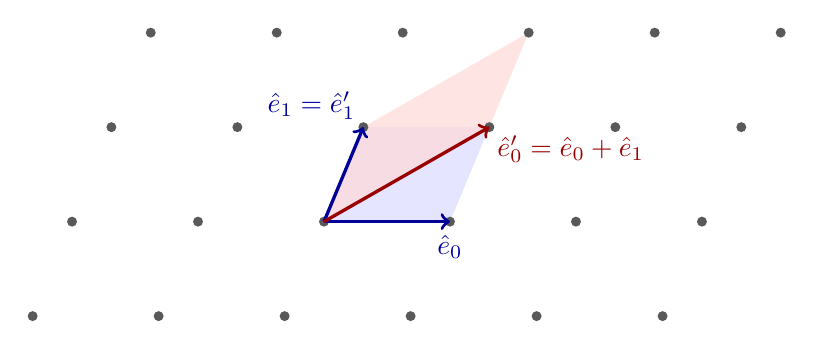
\begin{tikzpicture}[scale=1.0]
 \fill[blue!10] (0,0)--(1.6,0)--(2.1,1.2)--(0.5,1.2)--cycle;
 \fill[red!15,opacity=0.7] (0,0)--(2.1,1.2)--(2.6,2.4)--(0.5,1.2)--cycle;
 \foreach \i in {-2,...,3} \foreach \j in {-1,...,2}
   \fill[black!65] ({1.6*\i+0.5*\j},{1.2*\j}) circle (1.8pt);
 \draw[->,very thick,blue!60!black] (0,0)--(1.6,0) node[below=1pt] {$\hat e_0$};
 \draw[->,very thick,blue!60!black] (0,0)--(0.5,1.2)
   node[above left=-1pt] {$\hat e_1=\hat e_1'$};
 \draw[->,very thick,red!60!black] (0,0)--(2.1,1.2)
   node[below right=-1pt] {$\hat e_0'=\hat e_0+\hat e_1$};
\end{tikzpicture}
\caption{One lattice, two bases. The basis $(\hat e_0',\hat e_1')$ is obtained from
$(\hat e_0,\hat e_1)$ by $A=\left(\begin{smallmatrix}1&1\\0&1\end{smallmatrix}\right)\in
GL(2,\Z)$. The two shaded cells have the same area and define the same torus. The Gram
matrices of the two bases are $G$ and $G'=AGA^{\mathsf T}$; the element $L_A$ of $\Odd{2}$
records how winding and momentum numbers are relabelled.}
\label{fig:odd:basis}
\end{figure}

\subsection{Factorized dualities}

Let $e_k$ be the $d\times d$ matrix whose only non-zero entry is a $1$ in position $(k,k)$.
The \emph{factorized duality}\index{factorized duality} along the $k$-th circle is
\begin{equation}\label{eq:odd:factorized}
 D_k=\begin{pmatrix}\mathbf 1-e_k&e_k\\ e_k&\mathbf 1-e_k\end{pmatrix}
\end{equation}
\source{GPR §2.4, eq.~(2.4.29), ll.~1399--1414}. It is symmetric, so here the two
conventions of the pitfall box agree. \emph{Membership:} the matrix $e_k$ is a symmetric
projector, $e_k^2=e_k$, hence $e_k(\mathbf 1-e_k)=0$ and
$(\mathbf 1-e_k)^2=\mathbf 1-e_k$. The conditions \eqref{eq:odd:conditions} become
$2(\mathbf 1-e_k)e_k=0$ (twice) and $(\mathbf 1-e_k)^2+e_k^2=\mathbf 1$. The same
identities give
\begin{equation}\label{eq:odd:Dsquare}
 D_k^2=\begin{pmatrix}(\mathbf 1-e_k)^2+e_k^2&2(\mathbf 1-e_k)e_k\\
 2e_k(\mathbf 1-e_k)&e_k^2+(\mathbf 1-e_k)^2\end{pmatrix}=\mathbf 1,
 \qquad D_kD_l=D_lD_k ,
\end{equation}
the second because diagonal matrices commute. \emph{Action on the charges:} $D_k$ exchanges
$m^k$ with $n_k$ and leaves the other $2d-2$ charges alone. \emph{Action on the background:}
take $k=0$ and split the indices as $i=(0,\alpha)$. Then in \eqref{eq:odd:fractional}
\[
 a^{\mathsf T}E+c^{\mathsf T}=(\mathbf 1-e_0)E+e_0
 =\begin{pmatrix}1&0\\E_{\alpha0}&E_{\alpha\beta}\end{pmatrix},\qquad
 b^{\mathsf T}E+d^{\mathsf T}=e_0E+(\mathbf 1-e_0)
 =\begin{pmatrix}E_{00}&E_{0\beta}\\0&\mathbf 1\end{pmatrix}.
\]
The second matrix is upper triangular with inverse
$\left(\begin{smallmatrix}1/E_{00}&-E_{0\beta}/E_{00}\\0&\mathbf 1\end{smallmatrix}\right)$,
and $E_{00}=G_{00}>0$. Multiplying,
\begin{equation}\label{eq:odd:buscher}
 E'=\begin{pmatrix}\dfrac{1}{E_{00}}&-\dfrac{E_{0\beta}}{E_{00}}\\[3mm]
 \dfrac{E_{\alpha0}}{E_{00}}&E_{\alpha\beta}-\dfrac{E_{\alpha0}E_{0\beta}}{E_{00}}
 \end{pmatrix}.
\end{equation}
These are the Buscher rules\index{Buscher rules} of \cref{ch:buscher} in their compact
form, up to the sign of the two mixed entries. For a product background,
$E_{0\beta}=E_{\alpha0}=0$ and $E_{00}=R^2/\ap$, \eqref{eq:odd:buscher} is
$R^2/\ap\mapsto\ap/R^2$ with the other directions untouched: $D_k$ is the circle duality of
\cref{ch:tduality} performed on one circle \source{GPR §2.4, ll.~1419--1421}.

\begin{remark}[The sign of the mixed entries]\label{rem:odd:sign}
\Cref{ch:buscher} uses the matrix $T_\theta$, which is $D_0$ with $e_0$ replaced by $-e_0$
in the off-diagonal blocks, and finds \eqref{eq:odd:buscher} with the opposite sign in the
first row and the first column. The two are related by a basis change: for the reflection
$r_0=\mathbf 1-2e_0\in GL(d,\Z)$ of the dualized coordinate one has
$(\mathbf 1-e_0)r_0=\mathbf 1-e_0$ and $e_0r_0=-e_0$, hence
\begin{equation}\label{eq:odd:Ttheta}
 T_\theta=D_0\,L_{r_0}.
\end{equation}
By \eqref{eq:odd:basisaction}, $L_{r_0}$ flips the sign of exactly the entries
$E_{0\beta}$ and $E_{\alpha0}$. So the two forms of the rules differ by the orientation of
the dual circle, which is a matter of convention, and both $D_0$ and $T_\theta$ belong to
$\Odd{d}$. Since \eqref{eq:odd:buscher} was derived for every $d$ from
\cref{thm:odd:action}, this also proves for every $d$ the statement of \cref{ch:buscher}
that the Buscher rules are the conjugation $\HH\mapsto T_\theta^{\mathsf T}\HH\,T_\theta$.
\end{remark}

\emph{Physical meaning.} Unlike the first two families, $D_k$ is not a symmetry of the
classical sigma-model action under a change of variables that a point particle could
follow. It exchanges a Kaluza--Klein momentum with a winding number, and only an extended
object has winding. The argument that it is a symmetry is either the spectrum
(\cref{thm:odd:spectrum}), or the worldsheet path integral of \cref{ch:buscher}, or the
enhanced gauge symmetry at the self-dual radius (\cref{ch:tduality}).

\begin{proposition}[All circles at once]\label{prop:odd:product}
$D_0D_1\cdots D_{d-1}=\eta$. Consequently $\eta^{\mathsf T}\HH(G,0)\,\eta=\HH(G^{-1},0)$:
dualizing every circle of a torus without $B$-field inverts the metric.
\end{proposition}
\begin{proof}
Let $\hat e_k=\diag(e_k,e_k)$. These are commuting projectors with
$\hat e_k\hat e_l=0$ for $k\neq l$ and $\sum_k\hat e_k=\mathbf 1$, they commute with
$\eta$, and $D_k=\mathbf 1+\hat e_k(\eta-\mathbf 1)$. In the product
$\prod_k\big(\mathbf 1+\hat e_k(\eta-\mathbf 1)\big)$ every term containing two different
projectors vanishes, leaving $\mathbf 1+\sum_k\hat e_k(\eta-\mathbf 1)=\eta$. For the
second statement put $g=\eta$ in \eqref{eq:odd:fractional}: $a=d=0$, $b=c=\mathbf 1$ and
$E'=E^{-1}$, which for $B=0$ is $G'=G^{-1}$.
\end{proof}
For general $B$ the full duality is $E\mapsto E^{-1}$, the direct generalization of
$R^2/\ap\mapsto\ap/R^2$; the symmetric part of $E^{-1}$ is
$(G-BG^{-1}B)^{-1}$, not $G^{-1}$ (\cref{ex:odd:Einv}).

\Cref{tab:odd:generators} collects the three families.

\begin{table}[t]
\centering\small
\begin{tabular}{@{}l@{\hspace{6pt}}l@{\hspace{6pt}}l@{\hspace{6pt}}l@{\hspace{6pt}}l@{}}\toprule
 & matrix $g$ & background & $(m,n)\mapsto$ & origin\\\midrule
$B$-shift & $S_\Theta=\left(\begin{smallmatrix}\mathbf 1&0\\-\Theta&\mathbf 1
 \end{smallmatrix}\right)$ & $B\mapsto B+\Theta$ & $(m,\;n-\Theta m)$ & large gauge transf.\\[4pt]
basis change & $L_A=\left(\begin{smallmatrix}A^{\mathsf T}&0\\0&A^{-1}
 \end{smallmatrix}\right)$ & $E\mapsto AEA^{\mathsf T}$ & $(A^{\mathsf T}m,\;A^{-1}n)$ &
 large diffeomorphism\\[4pt]
fact.\ duality & $D_k=\left(\begin{smallmatrix}\mathbf 1-e_k&e_k\\e_k&\mathbf 1-e_k
 \end{smallmatrix}\right)$ & rules \eqref{eq:odd:buscher} &
 $m^k\leftrightarrow n_k$ & stringy, $R_k\to\ap/R_k$\\\bottomrule
\end{tabular}
\caption{The three families of elements of $\Odd{d}$, in the convention
$\HH\mapsto g^{\mathsf T}\HH g$, $Z=(m,n)\mapsto gZ$. Here $\Theta$ is an antisymmetric
integer matrix and $A\in GL(d,\Z)$.}
\label{tab:odd:generators}
\end{table}

%=====================================================================================
\section{Worked example: \texorpdfstring{$d=2$}{d=2} with explicit
 \texorpdfstring{$4\times4$}{4x4} matrices}\label{sec:odd:example}

For $T^2$ the charge vector is $Z=(m^0,m^1;n_0,n_1)$ and
$\frac12Z^{\mathsf T}\eta Z=m^0n_0+m^1n_1$. There is one independent $B$-shift, generated by
$\Theta=\varepsilon=\left(\begin{smallmatrix}0&1\\-1&0\end{smallmatrix}\right)$, and we
take $A=\left(\begin{smallmatrix}1&1\\0&1\end{smallmatrix}\right)$ of
\cref{fig:odd:basis} as a sample basis change. From \eqref{eq:odd:shift},
\eqref{eq:odd:basis} and \eqref{eq:odd:factorized}:
\begin{equation}\label{eq:odd:4x4}
\begin{gathered}
 S_\varepsilon=\begin{pmatrix}1&0&0&0\\0&1&0&0\\0&-1&1&0\\1&0&0&1\end{pmatrix},\qquad
 L_A=\begin{pmatrix}1&0&0&0\\1&1&0&0\\0&0&1&-1\\0&0&0&1\end{pmatrix},\\[2mm]
 D_0=\begin{pmatrix}0&0&1&0\\0&1&0&0\\1&0&0&0\\0&0&0&1\end{pmatrix},\qquad
 D_1=\begin{pmatrix}1&0&0&0\\0&0&0&1\\0&0&1&0\\0&1&0&0\end{pmatrix},\qquad
 D_0D_1=\begin{pmatrix}0&0&1&0\\0&0&0&1\\1&0&0&0\\0&1&0&0\end{pmatrix}=\eta .
\end{gathered}
\end{equation}
The reader should check one of them against \eqref{eq:odd:def} by hand; for $S_\varepsilon$,
for instance, $\eta S_\varepsilon$ has rows $(0,-1,1,0)$, $(1,0,0,1)$, $(1,0,0,0)$,
$(0,1,0,0)$, and multiplying by $S_\varepsilon^{\mathsf T}$ from the left returns $\eta$.
On the charges,
$S_\varepsilon Z=(m^0,m^1;\,n_0-m^1,\,n_1+m^0)$ and
$L_AZ=(m^0,\,m^0+m^1;\,n_0-n_1,\,n_1)$, and one verifies directly that both preserve
$m^0n_0+m^1n_1$: for $S_\varepsilon$ the two new terms are $-m^0m^1+m^1m^0=0$.

\paragraph{A background with numbers.} Take a rectangular torus with radii
$R_0=2\sqrt{\ap}$ and $R_1=\sqrt{\ap}$ and half a unit of $B$-field:
\begin{equation}\label{eq:odd:exbackground}
 G=\begin{pmatrix}4&0\\0&1\end{pmatrix},\quad
 B=\tfrac12\varepsilon,\quad
 E=\begin{pmatrix}4&\tfrac12\\-\tfrac12&1\end{pmatrix},\quad
 \HH=\begin{pmatrix}\tfrac{17}{4}&0&0&\tfrac12\\[1pt]0&\tfrac{17}{16}&-\tfrac18&0\\[1pt]
 0&-\tfrac18&\tfrac14&0\\[1pt]\tfrac12&0&0&1\end{pmatrix}.
\end{equation}
The blocks of $\HH$ follow from $BG^{-1}B=-\diag(\frac1{4},\frac1{16})$, so that
$G-BG^{-1}B=\diag(\frac{17}4,\frac{17}{16})$, and from
$BG^{-1}=\left(\begin{smallmatrix}0&1/2\\-1/8&0\end{smallmatrix}\right)$. As a check,
\eqref{eq:odd:squares} gives the same quadratic form:
$\frac14(n_0-\frac12m^1)^2+(n_1+\frac12m^0)^2+4(m^0)^2+(m^1)^2$.

Now dualize the circle of radius $R_0$. From \eqref{eq:odd:buscher} with $E_{00}=4$,
$E_{01}=\frac12$, $E_{10}=-\frac12$, $E_{11}=1$:
\begin{equation}\label{eq:odd:exdual}
 E'=\begin{pmatrix}\tfrac14&-\tfrac18\\[2pt]-\tfrac18&1+\tfrac1{16}\end{pmatrix}
 =G',\qquad B'=0 .
\end{equation}
The dual torus has no $B$-field at all. Its first circle has radius
$\sqrt{\ap}/2=\ap/R_0$, as expected, and its two cycles are no longer orthogonal: the angle
$\vartheta$ between them satisfies
$\cos\vartheta=G'_{01}/\sqrt{G'_{00}G'_{11}}=-\frac18\big/\sqrt{\tfrac{17}{64}}
=-1/\sqrt{17}$, so $\vartheta\approx104^\circ$. \emph{The $B$-field of one description is
the tilt of the torus in the other.} The generalized metric of the dual background can be
computed in two ways, from \eqref{eq:odd:exdual} and \eqref{eq:odd:Heta}, or as
$D_0\HH D_0$, which exchanges the first and third rows and columns of
\eqref{eq:odd:exbackground}; both give
\[
 \HH'=\begin{pmatrix}\tfrac14&-\tfrac18&0&0\\[1pt]-\tfrac18&\tfrac{17}{16}&0&0\\[1pt]
 0&0&\tfrac{17}4&\tfrac12\\[1pt]0&0&\tfrac12&1\end{pmatrix},\qquad
 G'^{-1}=\begin{pmatrix}\tfrac{17}4&\tfrac12\\[1pt]\tfrac12&1\end{pmatrix},\quad
 \det G'=\tfrac14 .
\]
\Cref{tab:odd:example} lists a few states. Each row is one instance of
\eqref{eq:odd:spectrum}.

\begin{table}[t]
\centering\small
\begin{tabular}{@{}ccccc@{}}\toprule
charge $Z$ on the dual torus & $Z^{\mathsf T}\HH'Z$ & $D_0Z$ on the original torus &
$(D_0Z)^{\mathsf T}\HH(D_0Z)$ & $N-\tilde N$\\\midrule
$(1,0;0,0)$ & $\frac14$ & $(0,0;1,0)$ & $\frac14$ & $0$\\[2pt]
$(0,0;1,0)$ & $\frac{17}4$ & $(1,0;0,0)$ & $\frac{17}4$ & $0$\\[2pt]
$(0,1;1,0)$ & $\frac{85}{16}$ & $(1,1;0,0)$ & $\frac{85}{16}$ & $0$\\[2pt]
$(1,0;1,0)$ & $\frac92$ & $(1,0;1,0)$ & $\frac92$ & $1$\\[2pt]
$(1,1;0,1)$ & $\frac{33}{16}$ & $(0,1;1,1)$ & $\frac{33}{16}$ & $1$\\\bottomrule
\end{tabular}
\caption{States of the background \eqref{eq:odd:exbackground} and of its dual
\eqref{eq:odd:exdual}, with $Z=(m^0,m^1;n_0,n_1)$. A string wound once around the small
circle of the dual torus (first row) is a string with one unit of momentum on the large
circle of the original torus. With the oscillators, $\ap M^2$ is the second column plus
$2(N+\tilde N-2)$; for the fourth row the lightest state has $N=1$, $\tilde N=0$ and
$\ap M^2=\frac52$ in both descriptions.}
\label{tab:odd:example}
\end{table}

\paragraph{The elements do not commute.} Conjugating the $B$-shift by the duality gives
\begin{equation}\label{eq:odd:mirror}
 D_0\,S_\varepsilon\,D_0=\begin{pmatrix}1&-1&0&0\\0&1&0&0\\0&0&1&0\\0&0&1&1\end{pmatrix}
 =L_{A'},\qquad A'=\begin{pmatrix}1&0\\-1&1\end{pmatrix},
\end{equation}
a basis change. In words: the stringy periodicity $B_{01}\to B_{01}+1$ of the original
torus is, in the dual description, the geometric fact that the lattice of the dual torus
can be described in a sheared basis. This is visible in the example: shifting
$B=\frac12\varepsilon$ to $\frac32\varepsilon$ changes the off-diagonal entry of $G'$ from
$-\frac18$ to $-\frac38$ and $G'_{11}$ from $\frac{17}{16}$ to $\frac{25}{16}$, which is
the change of basis $\hat e'_1\to\hat e'_1-\hat e'_0$ of the dual lattice
($G'_{01}-G'_{00}=-\frac38$, $G'_{11}-2G'_{01}+G'_{00}=\frac{25}{16}$). Since $D_0S_\varepsilon D_0\neq
S_\varepsilon$, the group is not abelian, and the element $D_0S_\varepsilon$ has infinite
order. Relation \eqref{eq:odd:mirror} is the matrix form of the exchange of the K\"ahler and
complex-structure moduli of $T^2$, the simplest example of mirror symmetry
(\cref{ch:torus2}).

%=====================================================================================
\section{The whole group, and what lies outside it}\label{sec:odd:generation}

\subsection{Relations and generation}

Within each family the composition law is simple. From the block forms one finds
\begin{equation}\label{eq:odd:relations}
 S_\Theta S_{\Theta'}=S_{\Theta+\Theta'},\qquad L_AL_{A'}=L_{A'A},\qquad
 L_A^{-1}S_\Theta L_A=S_{A\Theta A^{\mathsf T}},\qquad
 L_\pi D_kL_\pi^{-1}=D_{\pi(k)},
\end{equation}
where in the last relation $\pi$ is a permutation matrix (the labelling of $\pi(k)$ depends
on the convention for permutation matrices). So the $B$-shifts form an abelian group
isomorphic to $\Z^{d(d-1)/2}$, the basis changes form a copy of $GL(d,\Z)$, the basis
changes normalize the shifts, and all factorized dualities are conjugate to $D_0$.
Elements of the form $S_\Theta L_A$ make up the \emph{geometric
subgroup}\index{geometric subgroup}: they map a torus with a $B$-field to the same torus
in other coordinates and another gauge (\cref{ex:odd:geometric}). Everything that is
specific to strings comes from a single additional element, $D_0$.

\begin{theorem}[Generation]\label{thm:odd:generation}
The integer $B$-shifts $S_\Theta$, the basis changes $L_A$ and the factorized dualities
$D_k$ generate $\Odd{d}$. \TL\ \source{GPR §2.4, ll.~1422--1423}
\end{theorem}
Aldazabal, Marqu\'es and N\'u\~nez state the corresponding decomposition for the continuous
group, where $A$ ranges over $GL(d,\R)$ and $\Theta$ over real antisymmetric matrices
\source{AMN §3.1, eq.~(3.10), ll.~660--717}. Neither source proves the statement on the
page, and it is not formalized in the Lean development; we use it only as Tier~L
background. Nothing proved in this chapter depends on it: \cref{thm:odd:spectrum} holds for
every element of the group, whether or not it has been written as a product of generators.
For $d=1$ the theorem is a consequence of \cref{ex:odd:d1}: there are no shifts,
$GL(1,\Z)=\{\pm1\}$ gives $L_{-1}=-\mathbf 1$, $D_0=\eta$, and these two elements generate
the four elements of \eqref{eq:odd:O11Z}. For $d=2$ the group is described in
\cref{ch:torus2}.

A word on the list of families. With the action $\HH\mapsto g^{\mathsf T}\HH g$ the matrix
$g_\Theta$ of \eqref{eq:odd:shift}, with $\Theta$ in the upper right block, is also in the
group, but it does not shift $B$. From \eqref{eq:odd:fractional},
$E'=E(\Theta^{\mathsf T}E+\mathbf 1)^{-1}$, that is
\begin{equation}\label{eq:odd:beta}
 E'^{-1}=E^{-1}-\Theta ,\qquad g_\Theta=\eta\,S_{-\Theta}\,\eta .
\end{equation}
It is a $B$-shift conjugated by the full duality: it shifts the antisymmetric part of
$E^{-1}$. In double field theory such elements are called
$\beta$-transformations\index{beta-transformation@$\beta$-transformation} \source{AMN §3.1,
ll.~721--723}. They are not a fourth family of generators, since $\eta=D_0\cdots D_{d-1}$.

\subsection{What is not in the group}

\emph{Worldsheet parity.}\index{worldsheet parity} Reversing the orientation of the string,
$\sigma\to-\sigma$, maps $B\to-B$. On the doubled charges this is
$\Omega=\diag(\mathbf 1,-\mathbf 1)$, and indeed
$\Omega^{\mathsf T}\HH(G,B)\,\Omega=\HH(G,-B)$. But
$\Omega^{\mathsf T}\eta\,\Omega=-\eta$: parity exchanges left- and right-movers and flips
the sign of $n\cdot m$, so it is not an element of $\Odd{d}$ \source{GPR §2.4,
ll.~1423--1427}. It is a symmetry of the bosonic string, of a different kind, exchanging
$N$ with $\tilde N$.

\emph{Continuous transformations.} A generic element of $\OddR{d}$ is not a symmetry. It
maps a background to a physically different one, and this is how the real group sweeps out
the space of all backgrounds: by \cref{thm:odd:action} and \cref{ch:narain},
\begin{equation}\label{eq:odd:moduli}
 \mathcal M_d=\Odd{d}\,\backslash\,\OddR{d}\,/\,\big(O(d)\times O(d)\big),\qquad
 \dim\mathcal M_d=d(2d-1)-2\cdot\tfrac12d(d-1)=d^2 ,
\end{equation}
the $d^2$ being the components of $E=G+B$ \source{GPR §2.4, ll.~1263--1266}. The real
group acts on the space of backgrounds; the integer subgroup tells us which points of that
space are the same theory. Double field theory, a classical field theory, works with the
continuous group: Aldazabal, Marqu\'es and N\'u\~nez drop the $\Z$ as ``irrelevant for our
purposes of introducing DFT at the classical level'' \source{AMN §3.1, ll.~569--572}.
Integrality is a property of the quantum spectrum of charged states, which knows that $Z$
is an integer vector.

\emph{Fixed points.} An element $g\neq\pm\mathbf 1$ may fix a particular background,
$g^{\mathsf T}\HH g=\HH$. Then $e(Z)=gZ$ is a symmetry acting \emph{within} one theory, and
states are permuted among themselves. The self-dual circle $G=1$, fixed by $\eta$, is the
basic example (\cref{ch:tduality}); such points are the orbifold points of $\mathcal M_d$,
and they are where extra massless states appear.

%=====================================================================================
\section{What the machine has checked}\label{sec:odd:lean}

The three files \lean{DualScaleStream2/TDuality/ODD.lean}, \lean{Factorized.lean} and
\lean{Spectrum.lean} formalize the algebra of this chapter for arbitrary $d$, over Mathlib's
block matrices. The index type of a charge vector is the disjoint union
\lean{Fin d ⊕ Fin d}, so a charge vector is a function \lean{Charge d → ℤ} and
\lean{fromBlocks a b c d} is the block matrix \eqref{eq:odd:blocks}. The doc-comments of
\lean{ODD.lean} call the two halves ``momenta'' and ``windings'' in that order, whereas
\lean{GeneralizedMetric.lean} lists windings first, as we do. For the theorems of
\lean{ODD.lean} and \lean{Factorized.lean} the order does not matter, because $\eta$ and
$D_k$ are unchanged when the two halves are exchanged; it matters only for the
interpretation of \lean{thetaShift}, discussed below. All theorems quoted here depend only
on the standard axioms \lean{propext}, \lean{Classical.choice} and \lean{Quot.sound}.

\begin{leanbox}[The group as a predicate; closure under product and inverse]
\begin{leancode}
abbrev Charge (d : ℕ) := Fin d ⊕ Fin d
def eta (d : ℕ) : Matrix (Charge d) (Charge d) ℤ := fromBlocks 0 1 1 0
def IsODD (g : Matrix (Charge d) (Charge d) ℤ) : Prop :=
  gᵀ * eta d * g = eta d

theorem eta_mul_self : eta d * eta d = 1 := by ...
theorem eta_isODD : IsODD (eta d) := by ...
theorem isODD_mul (g h : Matrix (Charge d) (Charge d) ℤ)
    (hg : IsODD g) (hh : IsODD h) : IsODD (g * h) := by ...
theorem isODD_left_inv (g : Matrix (Charge d) (Charge d) ℤ) (hg : IsODD g) :
    (eta d * gᵀ * eta d) * g = 1 := by ...
theorem isODD_right_inv (g : Matrix (Charge d) (Charge d) ℤ) (hg : IsODD g) :
    g * (eta d * gᵀ * eta d) = 1 := by ...
theorem isODD_inv_isODD (g : Matrix (Charge d) (Charge d) ℤ) (hg : IsODD g) :
    IsODD (eta d * gᵀ * eta d) := by ...
\end{leancode}
\textbf{Reading.} \lean{IsODD g} is \eqref{eq:odd:def} for an integer matrix. The six
theorems are items (i)--(iv) of \cref{prop:odd:group}: $\eta^2=\mathbf 1$; $\eta$ is in the
group; products stay in the group; $\eta g^{\mathsf T}\eta$ is a left and a right inverse of
$g$ with integer entries by construction; and that inverse is in the group.
\textbf{What is not there.} The group is a predicate on matrices. No \lean{Group} or
\lean{Subgroup} structure is declared, the identity matrix is not shown to satisfy
\lean{IsODD} by a named theorem, and $\det g=\pm1$ and the closure under transposition are
not stated (\cref{ex:odd:leantranspose}).
\textbf{Proof idea.} \lean{isODD\_mul} is the \lean{calc} chain of our proof of (ii).
\lean{isODD\_left\_inv} regroups $(\eta g^{\mathsf T}\eta)g=\eta(g^{\mathsf T}\eta g)$ and
rewrites with the hypothesis and \lean{eta\_mul\_self}; the right inverse follows from
Mathlib's \lean{mul\_eq\_one\_comm} for square matrices over a commutative ring. \TA
\end{leanbox}

\begin{leanbox}[The three families are in the group]
\begin{leancode}
def thetaShift (Θ : Matrix (Fin d) (Fin d) ℤ) :
    Matrix (Charge d) (Charge d) ℤ := fromBlocks 1 Θ 0 1
def basisChange (A B : Matrix (Fin d) (Fin d) ℤ) :
    Matrix (Charge d) (Charge d) ℤ := fromBlocks A 0 0 B
def proj (k : Fin d) : Matrix (Fin d) (Fin d) ℤ := single k k 1
def factorized (k : Fin d) : Matrix (Charge d) (Charge d) ℤ :=
  fromBlocks (1 - proj k) (proj k) (proj k) (1 - proj k)

theorem thetaShift_isODD (Θ : Matrix (Fin d) (Fin d) ℤ) (hΘ : Θᵀ = -Θ) :
    IsODD (thetaShift Θ) := by ...
theorem basisChange_isODD (A B : Matrix (Fin d) (Fin d) ℤ)
    (h : Aᵀ * B = 1) : IsODD (basisChange A B) := by ...
theorem factorized_isODD (k : Fin d) : IsODD (factorized k) := by ...
theorem factorized_mul_self (k : Fin d) :
    factorized k * factorized k = 1 := by ...
theorem factorized_comm (k l : Fin d) :
    factorized k * factorized l = factorized l * factorized k := by ...
theorem factorized_two : factorized (0 : Fin 2) * factorized 1 = eta 2 := by ...
\end{leancode}
\textbf{Reading.} \lean{thetaShift Θ} is $g_\Theta$ of \eqref{eq:odd:shift}, and
$S_\Theta$ is its transpose; \lean{basisChange A B} is $\diag(A,B)$, and
$L_A=$ \lean{basisChange Aᵀ A⁻¹}; \lean{factorized k} is $D_k$. The first three theorems
are one direction each: \emph{if} $\Theta$ is antisymmetric then $g_\Theta$ is in the
group, \emph{if} $A^{\mathsf T}B=\mathbf 1$ then $\diag(A,B)$ is; the converses shown
in \cref{sec:odd:generators} are not formalized. The hypothesis
$A^{\mathsf T}B=\mathbf 1$ replaces the matrix inverse, so $GL(d,\Z)$ never has to be
mentioned. The next two are \eqref{eq:odd:Dsquare}. The last is \cref{prop:odd:product}
for $d=2$ only; the statement for general $d$ is not formalized
(\cref{ex:odd:leanproduct}). The physical readings attached to these matrices (large gauge
transformation, change of coordinates, $R\to\ap/R$) are in the doc-comments, not in the
statements, and are not Tier~A. In particular no Lean theorem in these three files says
that $g_\Theta$ shifts $B$; that is \lean{genMetric\_bshift} in \lean{DFT/BShift.lean},
which states
$g_\Theta\,\HH(G,B)\,g_\Theta^{\mathsf T}=\HH(G,B+\Theta)$ over $\R$, the
convention of GPR, equivalent to our \eqref{eq:odd:shiftaction} because
$S_\Theta=g_\Theta^{\mathsf T}$ (\cref{ch:genmetric}).
\textbf{Proof idea.} Unfold to \lean{fromBlocks}, multiply blockwise with
\lean{fromBlocks\_multiply}, and compare the four blocks. For $D_k$ the only input is
$e_k^2=e_k$ (\lean{proj\_mul\_self}, from Mathlib's algebra of matrix units), after which
\lean{abel} closes each block. \lean{factorized\_two} is a comparison of two explicit
$4\times4$ integer matrices, the last matrix in \eqref{eq:odd:4x4}, entry by entry
(\lean{fin\_cases}, \lean{rfl}). \TA
\end{leanbox}

\begin{leanbox}[The charge norm: even and invariant]
\begin{leancode}
def chargeNorm (Z : Charge d → ℤ) : ℤ := Z ⬝ᵥ (eta d *ᵥ Z)

theorem chargeNorm_sumElim (n w : Fin d → ℤ) :
    chargeNorm (Sum.elim n w) = 2 * (n ⬝ᵥ w) := by ...
theorem chargeNorm_even (Z : Charge d → ℤ) : Even (chargeNorm Z) := by ...
theorem chargeNorm_invariant (g : Matrix (Charge d) (Charge d) ℤ)
    (hg : IsODD g) (Z : Charge d → ℤ) :
    chargeNorm (g *ᵥ Z) = chargeNorm Z := by ...
\end{leancode}
\textbf{Reading.} \lean{chargeNorm Z} is $Z^{\mathsf T}\eta Z$. If the two halves of $Z$
are $n$ and $w$, it equals $2\,n\cdot w$; it is even for every integer $Z$, which is the
evenness of the Narain lattice of \cref{ch:narain} for all $d$; and it does not change
under $Z\mapsto gZ$ with $g$ in the group. The last statement is the second equation in
\eqref{eq:odd:spectrum}. The converse found in \cref{sec:odd:setting}, that invariance for
all $Z$ forces $g^{\mathsf T}\eta g=\eta$, is not formalized.
\textbf{Proof idea.} For invariance, move $g$ across the dot product with Mathlib's
\lean{dotProduct\_mulVec} and \lean{vecMul\_mulVec}, which produces $g^{\mathsf T}\eta g$,
and rewrite with the hypothesis. \TA
\end{leanbox}

\begin{leanbox}[Spectrum equivalence]
\begin{leancode}
noncomputable def massForm (H : Matrix (Charge d) (Charge d) ℝ)
    (Z : Charge d → ℝ) : ℝ := Z ⬝ᵥ (H *ᵥ Z)
theorem massForm_covariant (g H : Matrix (Charge d) (Charge d) ℝ)
    (Z : Charge d → ℝ) :
    massForm (gᵀ * H * g) Z = massForm H (g *ᵥ Z) := by ...

noncomputable def toReal (g : Matrix (Charge d) (Charge d) ℤ) :
    Matrix (Charge d) (Charge d) ℝ := g.map (Int.cast : ℤ → ℝ)

theorem spectrum_equivalence (g : Matrix (Charge d) (Charge d) ℤ)
    (hg : IsODD g) (H : Matrix (Charge d) (Charge d) ℝ) :
    ∃ e : (Charge d → ℤ) ≃ (Charge d → ℤ), ∀ Z : Charge d → ℤ,
      massForm ((toReal g)ᵀ * H * toReal g) (fun i => (Z i : ℝ)) =
        massForm H (fun i => (e Z i : ℝ)) ∧
      chargeNorm (e Z) = chargeNorm Z := by ...
\end{leancode}
\textbf{Reading.} For every $d$, every integer $g$ with $g^{\mathsf T}\eta g=\eta$ and
every real $2d\times2d$ matrix $H$, there exists a bijection $e$ of the set of integer
charge vectors such that, for all $Z$, the number $Z^{\mathsf T}(g^{\mathsf T}Hg)Z$ equals
$e(Z)^{\mathsf T}H\,e(Z)$ and $e(Z)$ has the same charge norm as $Z$. This is
\cref{thm:odd:spectrum} word for word, including the generality in $H$: the matrix need
not be symmetric, positive or of the form $\HH(G,B)$. The symbol \lean{≃} is Lean's type of
bijections given together with their inverse, and \lean{toReal} and the casts
\lean{(Z i : ℝ)} are needed because the group and the charges live over $\Z$ while the
background lives over $\R$. The statement is existential; the proof supplies
$e(Z)=gZ$ with inverse $Z\mapsto(\eta g^{\mathsf T}\eta)Z$.
\textbf{What it does not say.} It does not mention oscillators, $\ap$, the mass formula
\eqref{eq:odd:mass} as a whole, the partition function or correlation functions, and it
does not say that $g^{\mathsf T}\HH(G,B)\,g$ is again a generalized metric.
\Cref{cor:odd:full}, \cref{lem:odd:char}, \cref{lem:odd:graph} and \cref{thm:odd:action}
are proved on the page only. (The ``only if'' half of \cref{lem:odd:char} has a partial
Lean counterpart, \lean{etaR\_genMetric\_sq} and \lean{genMetric\_symm} in
\lean{DFT/GeneralizedMetric.lean}; see \cref{ch:genmetric}.)
\textbf{Proof idea.} The bijection is assembled from \lean{isODD\_left\_inv} and
\lean{isODD\_right\_inv}. For the mass form one first shows that casting to $\R$ commutes
with the matrix--vector product (\lean{push\_cast}), then applies
\lean{massForm\_covariant}, which is \eqref{eq:odd:covariance} and needs no hypothesis on
$g$. The charge-norm half is \lean{chargeNorm\_invariant}. \TA
\end{leanbox}

Two further files of the same directory, treated in \cref{ch:torus2}, contain statements we
have used: \lean{thetaShift\_mul} and \lean{basisChange\_mul} are the first two relations
in \eqref{eq:odd:relations} (for $g_\Theta$ and $\diag(A,B)$). The theorem
\lean{mirror\_conjugates\_tauShift} is the relation \eqref{eq:odd:mirror}, stated as
$D_0\,\diag(A,B)\,D_0=g_\Theta^{\mathsf T}$ for one explicit pair of $2\times2$ matrices.
Finally \lean{eta\_one\_reindex} states that for $d=1$ the matrix $\eta$, reindexed from
\lean{Fin 1 ⊕ Fin 1} to \lean{Fin 2}, is equal to the matrix \lean{hyperbolicU} of the
hyperbolic plane $U$ of \cref{ch:lattices}.

\begin{center}\small
\begin{tabular}{@{}>{\raggedright\arraybackslash}p{0.44\textwidth}c
  >{\raggedright\arraybackslash}p{0.44\textwidth}@{}}
\toprule
Claim & Tier & Evidence\\
\midrule
$\eta^2=\mathbf 1$; closure of $\Odd{d}$ under product and inverse;
 $g^{-1}=\eta g^{\mathsf T}\eta$ & \TA & \lean{eta\_mul\_self}, \lean{isODD\_mul},
 \lean{isODD\_left\_inv}, \lean{isODD\_right\_inv}, \lean{isODD\_inv\_isODD}\\[2pt]
$g_\Theta$, $\diag(A,B)$ with $A^{\mathsf T}B=\mathbf 1$, $D_k$, $\eta$ lie in $\Odd{d}$
 & \TA & \lean{thetaShift\_isODD}, \lean{basisChange\_isODD}, \lean{factorized\_isODD},
 \lean{eta\_isODD}\\[2pt]
$D_k^2=\mathbf 1$, $D_kD_l=D_lD_k$; $D_0D_1=\eta$ for $d=2$ & \TA &
 \lean{factorized\_mul\_self}, \lean{factorized\_comm}, \lean{factorized\_two}\\[2pt]
$Z^{\mathsf T}\eta Z=2n\cdot w$ is even and $\Odd{d}$-invariant & \TA &
 \lean{chargeNorm\_sumElim}, \lean{chargeNorm\_even}, \lean{chargeNorm\_invariant}\\[2pt]
\Cref{thm:odd:spectrum}: bijection of charges matching mass form and charge norm & \TA &
 \lean{spectrum\_equivalence}\\[2pt]
$\det g=\pm1$; $g^{\mathsf T}\in\Odd{d}$; $D_0\cdots D_{d-1}=\eta$ for all $d$;
 \cref{lem:odd:char,lem:odd:graph}; \cref{thm:odd:action}; \cref{cor:odd:full} & --- &
 proved on the page; \eqref{eq:odd:fractional} also checked symbolically (sympy)\\[2pt]
The three families generate $\Odd{d}$ & \TL & GPR §2.4, ll.~1422--1423\\[2pt]
Equivalence of the full conformal field theories, not only of the spectra & \TL &
 GPR §2.4, ll.~1336--1348; \cref{ch:buscher}\\[2pt]
Identification of \lean{massForm} and \lean{chargeNorm} with the mass and level matching
 of a physical string & \TL & \cref{ch:narain}; never Tier~A\\
\bottomrule
\end{tabular}
\end{center}

%=====================================================================================
\begin{summarybox}
\begin{itemize}[leftmargin=*,itemsep=1pt]
\item With $Z=(m,n)$, the background enters the closed-string spectrum only through
 $Z^{\mathsf T}\HH(G,B)Z$ and level matching only through $\frac12Z^{\mathsf T}\eta Z
 =n\cdot m$. A relabelling $Z\mapsto gZ$ respects level matching for all charges if and
 only if $g^{\mathsf T}\eta g=\eta$.
\item $\Odd{d}$ is the group of integer matrices with $g^{\mathsf T}\eta g=\eta$. The
 inverse is $\eta g^{\mathsf T}\eta$, automatically an integer matrix; the transpose of an
 element is an element; $\det g=\pm1$. The real group has dimension $d(2d-1)$, and
 $O(1,1;\Z)=\{\pm\mathbf 1,\pm\eta\}$.
\item Spectrum equivalence: for $g\in\Odd{d}$ the map $Z\mapsto gZ$ is a bijection of the
 charge lattice with $Z^{\mathsf T}(g^{\mathsf T}\HH g)Z=(gZ)^{\mathsf T}\HH(gZ)$ and
 $(gZ)^{\mathsf T}\eta(gZ)=Z^{\mathsf T}\eta Z$. The proof is three lines, and it is the
 Lean theorem \lean{spectrum\_equivalence}.
\item A matrix is a generalized metric if and only if it is symmetric, positive definite and
 satisfies $\HH\eta\HH=\eta$. Hence $g^{\mathsf T}\HH(E)g=\HH(E')$ with
 $E'=(a^{\mathsf T}E+c^{\mathsf T})(b^{\mathsf T}E+d^{\mathsf T})^{-1}$.
\item Three families: integer $B$-shifts (large gauge transformations, $B\mapsto B+\Theta$,
 $n\mapsto n-\Theta m$); basis changes (large diffeomorphisms, $E\mapsto AEA^{\mathsf T}$);
 factorized dualities ($m^k\leftrightarrow n_k$, Buscher rules, $R_k\to\ap/R_k$). Their
 product over all circles is $\eta$, which acts as $E\mapsto E^{-1}$.
\item That these families generate the whole group is Tier~L and is not formalized.
 Worldsheet parity $B\to-B$ is not in the group, and a generic real element maps a
 background to an inequivalent one.
\end{itemize}
\end{summarybox}

%=====================================================================================
\section*{Exercises}
\addcontentsline{toc}{section}{Exercises}

\begin{exercise}[$\star$ Relations]\label{ex:odd:relations}
Verify the four relations \eqref{eq:odd:relations} by block multiplication. For the last
one take $d=3$ and the cyclic permutation, write $L_\pi$ and $D_0$ as $6\times6$
matrices, and find which $D_j$ results.
\end{exercise}

\begin{exercise}[$\star$ The table]\label{ex:odd:table}
For the background \eqref{eq:odd:exbackground}, apply $D_1$ instead of $D_0$. Compute $E'$
from \eqref{eq:odd:buscher} (with the roles of the indices $0$ and $1$ exchanged), show
that $B'=0$ again, and find the radii and the angle of the dual torus. Reproduce two rows
of the analogue of \cref{tab:odd:example}.
\end{exercise}

\begin{exercise}[$\star\star$ The full duality]\label{ex:odd:Einv}
Show that $\eta$ acts as $E\mapsto E^{-1}$, and that the symmetric and antisymmetric parts
of $E^{-1}=(G+B)^{-1}$ are $G'=(G-BG^{-1}B)^{-1}$ and $B'=-G^{-1}B\,(G-BG^{-1}B)^{-1}$.
(Hint: compare the blocks of $\eta\,\HH(G,B)\,\eta$ with those of $\HH(G',B')$.) Evaluate
both for the background \eqref{eq:odd:exbackground} and check the result against
$D_1$ applied to \eqref{eq:odd:exdual}.
\end{exercise}

\begin{exercise}[$\star\star$ The geometric subgroup]\label{ex:odd:geometric}
Show that the elements of $\Odd{d}$ with vanishing upper right block, $b=0$, are exactly
the products $S_\Theta L_A$ with $A\in GL(d,\Z)$ and $\Theta$ antisymmetric and integer, and
that they form a subgroup. Show that $S_\Theta L_A$ maps $(G,B)$ to
$(AGA^{\mathsf T},A(B+\Theta)A^{\mathsf T})$ (the shift acts first; why?), and conclude that a point particle on the torus,
whose spectrum is $n^{\mathsf T}G^{-1}n$, cannot distinguish the two backgrounds when
$B=0=\Theta$.
\end{exercise}

\begin{exercise}[$\star\star$ Which elements act trivially?]\label{ex:odd:trivial}
Show that $g^{\mathsf T}\HH g=\HH$ for \emph{all} generalized metrics $\HH$ if and only if
$g=\pm\mathbf 1$. (Hint: use $\HH(G,0)$ with diagonal $G$ first, then a non-diagonal $G$,
then $B\neq0$.) Conclude that the group acting faithfully on backgrounds is
$\Odd{d}/\{\pm\mathbf 1\}$, and describe it for $d=1$.
\end{exercise}

\begin{exercise}[$\star\star$ Infinitesimal transformations]\label{ex:odd:lie}
Let $X=\left(\begin{smallmatrix}\alpha&\beta\\ \gamma&-\alpha^{\mathsf T}
\end{smallmatrix}\right)$ with $\beta,\gamma$ antisymmetric. (a) Verify
$X^{\mathsf T}\eta+\eta X=0$. (b) Compute $\exp X$ when only $\gamma\neq0$ and when only
$\alpha\neq0$, and compare with $S_\Theta$ and $L_A$. (c) Using
\eqref{eq:odd:fractional} to first order, show that
$\delta E=\alpha^{\mathsf T}E+E\alpha+\gamma^{\mathsf T}-E\beta^{\mathsf T}E$. Which term
is non-linear in the background, and why does it carry the name
$\beta$-transformation?
\end{exercise}

\begin{exercise}[$\star\star$ Lean: the transpose]\label{ex:odd:leantranspose}
State and prove in Lean: \lean{theorem isODD\_transpose (g : Matrix (Charge d) (Charge d) ℤ)
(hg : IsODD g) : IsODD gᵀ}. Follow the proof of \cref{prop:odd:group}(iv): start from
\lean{isODD\_right\_inv g hg}, multiply on the right by \lean{eta d}, and simplify with
\lean{Matrix.mul\_assoc} and \lean{eta\_mul\_self}. Then deduce that $S_\Theta$ satisfies
\lean{IsODD} from \lean{thetaShift\_isODD}.
\end{exercise}

\begin{exercise}[$\star\star$ Lean: small elements]\label{ex:odd:leansmall}
State and prove \lean{IsODD (1 : Matrix (Charge d) (Charge d) ℤ)} and
\lean{IsODD (-1 : Matrix (Charge d) (Charge d) ℤ)}. Then obtain the second statement in a
different way, from \lean{basisChange\_isODD} with $A=B=-\mathbf 1$; you will need a lemma
saying that \lean{basisChange (-1) (-1) = -1}.
\end{exercise}

\begin{exercise}[$\star\star\star$ Lean: all circles at once]\label{ex:odd:leanproduct}
(a) Prove \lean{factorized (0 : Fin 3) * factorized 1 * factorized 2 = eta 3} in the style
of \lean{factorized\_two}. (b) Formulate \cref{prop:odd:product} for general $d$ in Lean.
One possibility uses \lean{Finset.noncommProd} together with \lean{factorized\_comm};
another avoids products altogether by proving
$D_k=\mathbf 1+\hat e_k(\eta-\mathbf 1)$ and an induction over a list of distinct indices.
Explain which hypotheses of the on-page proof each formulation needs.
\end{exercise}

\begin{exercise}[$\star\star\star$ Symmetries of the most symmetric torus]\label{ex:odd:fixed}
Let $\HH=\mathbf 1$, that is $G=\mathbf 1$, $B=0$: a product of $d$ self-dual circles.
(a) Show that an integer matrix $g$ with $g^{\mathsf T}g=\mathbf 1$ is a signed permutation
matrix, so that there are $2^{2d}(2d)!$ of them. (b) Show that such a $g$ lies in $\Odd{d}$
if and only if it commutes with $\eta$, and that there are $2^d\cdot2^d\cdot d!$ such
elements: $4$, $32$, $384$ for $d=1,2,3$. Identify the three factors with reflections of
circles, factorized dualities and permutations of circles. (c) For $d=2$ the permutation
matrix $g$ that exchanges $m^1$ with $n_0$ satisfies $g^{\mathsf T}\HH g=\HH$ but is not in
$\Odd{2}$. Which part of the proof of \cref{thm:odd:spectrum} fails for it? Exhibit a
charge $Z$ that is allowed at oscillator levels $N=\tilde N$ while $gZ$ is not. This shows
that preserving the form of $\HH$ is not enough; level matching is what singles out
$\Odd{d}$.
\end{exercise}

\section*{Further reading}
\addcontentsline{toc}{section}{Further reading}
\begin{itemize}[leftmargin=*,itemsep=2pt]
\item The definition of $O(d,d)$ in block form, the action on $E$ by fractional linear
 transformations, the three families with their physical interpretation, the generation
 statement and worldsheet parity: \source{GPR §2.4, ll.~1213--1427}. The transformation of
 the oscillators, which completes the map between the two Hilbert spaces:
 \source{GPR §2.4, ll.~1428--1497}.
\item The same group from the point of view of double field theory, with the generalized
 momentum, the decomposition into diffeomorphisms, shifts and factorized T-dualities, the
 Buscher rules and $\beta$-transformations: \source{AMN §3.1, ll.~567--779}.
\item The Lean sources are \lean{ODD.lean}, \lean{Factorized.lean} and
 \lean{Spectrum.lean} in the directory \lean{DualScaleStream2/TDuality/}; their headers list
 what is and what is not proved. For the real generalized metric see \lean{DualScaleStream2/DFT/GeneralizedMetric.lean}
 and \cref{ch:genmetric}; for $d=2$ see \cref{ch:torus2}.
\end{itemize}
